\documentclass[a4paper]{article}
\usepackage{mathtext}
\usepackage[russian]{babel}
\usepackage{indentfirst}
\usepackage[pdftex]{graphicx}
\usepackage{multirow}
\usepackage{csvsimple}
\usepackage[left=2cm,right=2cm,top=2cm,bottom=2cm]{geometry}
\title{Работа 2.2.6 Определение энергии активации по температурной зависимости вязкости жидкости}
\begin{document}
\maketitle
\section{Аннотация}
В работе проводится измерение скорости падения шариков из разных материалов в жидкости (глицерин) различной температуры. Затем по установившейся скорости при помощи формулы Стокса определяется вязкость жидкости и энергия активации молекул.
\section{Теоретические сведения}
Для перехода в новое состояние молекула должна получить энергию активации W. По формуле Больцмана 
\begin{equation}
\eta \sim Ae^{W/k T}
\end{equation}
Тогда график $Ln(\eta)$ в зависимости от $(1/T)$ - прямая, по угл. коэфф. можно определить W.

Для определения вязкости жидкости применим формулу Стокса:
\begin{equation}
F=6 \pi \eta r v
\label{stox}
\end{equation}

Найдём уравнение движения шарика в жидкости:
\begin{equation}
v (t) = v_{y} - [ v_{y} - v (0)] e^{-t/\tau}
\end{equation}

\begin{equation}
v_y = \frac{2}{9} g r^2 \frac{\rho - \rho_{ж}}{\eta}
\end{equation}

Отсюда вязкость равна
\begin{equation}
\eta = \frac{2}{9•} g r^2 \frac{\rho - \rho_{ж}}{v_y•}
\label{eq}
\end{equation}
Энергию активации молекул можно найти из равенства
\begin{equation}
W = k \frac{d ln(\eta)}{d(1/T)}
\label{nrg}
\end{equation}
где $k=1,38*10^{-23}$ - постоянная Больцмана
\section{Оборудование и инструментальные погрешности}

\begin{figure}[h]
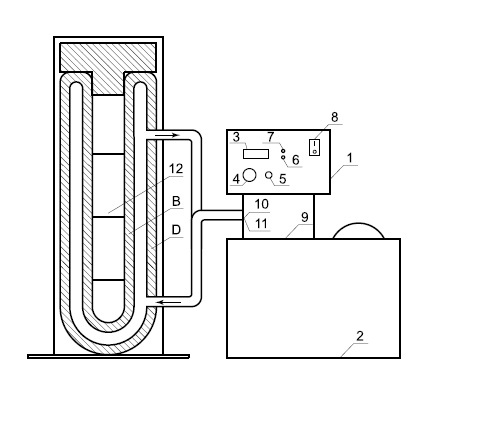
\includegraphics[scale=0.75]{5}
\caption{Установка для определения вязкости жидкости}
\label{pic}
\end{figure}

{\bf Линейка: } $\Delta = \pm 1 $ мм

{\bf Микроскоп с градуировкой: } $\Delta = \pm 0,05 $ мм

{\bf Термометр на термостате: } $\Delta = \pm 0,1 $ К

{\bf Секундомер: } $\Delta = \pm 0,1 $ с

Схема установки изображена на рисунке \ref{pic}


\section{Результаты измерений и обработка данных}
\subsection{Определение вязкости}
С помощью формулы \ref{eq} определим вязкость жидкости в зависимости от температуры. При расчётах учтём зависимость плотности глицерина от 
температуры. При оценке погрешностей используем формулу:
\begin{equation}
\sigma_\eta = \eta \sqrt{(\frac{\sigma_l}{l})^{2} + (\frac{\sigma_t}{t})^{2} +  4 (\frac{\sigma_r}{r})^{2}}
\end{equation}

Расчёты проведены в системе единиц СГС: 1 Па*с = 10 пуаз.
\begin{table}[h]
\begin{tabular}{|l|l|l|l|l|l|}
\hline
\multicolumn{1}{|r|}{\textbf{Температура, С}} & \textbf{23.2} & \textbf{30.1} & \textbf{40.0} & \textbf{50.0}  & \textbf{60.0}  \\ \hline
\textbf{Вязкость 1 опыт, пуаз}                & 4.5$\pm$0.2       & 2.7$\pm$0.1       & 1.6$\pm$0.1       & 0.94$\pm$0.05      & 0.58$\pm$0.03      \\ \hline
\textbf{Вязкость 2 опыт, пуаз}                & 3.9$\pm$0.5       & 2.$\pm$.1       & 1.4$\pm$0.1       & 0.91$\pm$0.05      & 0.50$\pm$0.03      \\ \hline
\textbf{Вязкость 3 опыт, пуаз}                & 4.3$\pm$0.5       & 2.5$\pm$0.3       & 1.2$\pm$0.2       & 0.8$\pm$0.1        & 0.40$\pm$0.05      \\ \hline
\textbf{Вязкость 4 опыт, пуаз}                & 4.6$\pm$0.2       & 2.4$\pm$0.4       & 0.9$\pm$0.1       & 0.8$\pm$0.1        & 0.46$\pm$0.06      \\ \hline
\textbf{Средняя вязкость, пуаз}               & \textbf{4.24} & \textbf{2.57} & \textbf{1.29} & \textbf{0.845} & \textbf{0.475} \\ \hline
\end{tabular}
\end{table}

Можно заметить, что более высокие погрешности в 3-м и 4-м опытах; это связано с малым размером металлического шарика.
\subsection{Определение чисел Рейнольдса; оценка времени и пути релаксации}
Число Рейнольдса можно определить следующим образом:
\begin{equation}
Re=\frac{v R \rho}{\eta}
\end{equation}, где $v$ - характерная скорость течения, $R$ - радиус шарика, $\rho$ - плотность жидкости, а $\eta$ - вычисленный нами коэффициент вязкости. Найдём $Re$ для каждой температуры. Результаты в таблице \ref{re}.
\begin{table}[h]
\begin{tabular}{llllll}
\hline
\multicolumn{1}{|r|}{\textbf{Температура, С}} & \multicolumn{1}{l|}{\textbf{23.2}} & \multicolumn{1}{l|}{\textbf{30.1}} & \multicolumn{1}{l|}{\textbf{40.0}} & \multicolumn{1}{l|}{\textbf{50.0}} & \multicolumn{1}{l|}{\textbf{60.0}} \\ \hline
\multicolumn{1}{|l|}{\textbf{Re, опыт 1}}     & \multicolumn{1}{l|}{0.024}         & \multicolumn{1}{l|}{0.057}         & \multicolumn{1}{l|}{0.18}          & \multicolumn{1}{l|}{0.48}          & \multicolumn{1}{l|}{1.4}           \\ \hline
\multicolumn{1}{|l|}{\textbf{Re, опыт 2}}     & \multicolumn{1}{l|}{0.0072}        & \multicolumn{1}{l|}{0.059}         & \multicolumn{1}{l|}{0.21}          & \multicolumn{1}{l|}{0.59}          & \multicolumn{1}{l|}{1.4}           \\ \hline
\multicolumn{1}{|l|}{\textbf{Re, опыт 3}}     & \multicolumn{1}{l|}{0.0086}        & \multicolumn{1}{l|}{0.025}         & \multicolumn{1}{l|}{0.070}         & \multicolumn{1}{l|}{0.23}          & \multicolumn{1}{l|}{0.82}          \\ \hline
\multicolumn{1}{|l|}{\textbf{Re, опыт 4}}     & \multicolumn{1}{l|}{0.023}         & \multicolumn{1}{l|}{0.013}         & \multicolumn{1}{l|}{0.077}         & \multicolumn{1}{l|}{0.12}          & \multicolumn{1}{l|}{0.53}          \\ \hline
\textbf{}                                     & \textbf{}                          & \textbf{}                          & \textbf{}                          & \textbf{}                          & \textbf{}                         
\end{tabular}
\caption{Числа Рейнольдса в каждом опыте}
\label{re}
\end{table}

Далее в таблице \ref{2} оценим время и путь релаксации по формулам 
\begin{equation}
\tau = \frac{V \rho}{6 \pi \eta r} = \frac{2 r^{2} \rho}{9 \eta}
\end{equation}
\begin{equation}
S_{уст} = V_{уст} * \tau
\end{equation}

% Please add the following required packages to your document preamble:
% \usepackage{multirow}
\begin{table}[h]
\begin{tabular}{|l|l|l|l|ll}
\cline{1-4}
\multicolumn{1}{|r|}{\textbf{Температура, С}} & \textbf{№ опыта} & \textbf{Время релаксации, $10^{-4}$ с} & \textbf{Путь релаксации, $10^{-4}$ см} & \textbf{} & \textbf{} \\ \cline{1-4}
\multirow{4}{*}{\textbf{23.2}}                & \textbf{1}       & 15                                  & 12                                 &           & \textbf{} \\ \cline{2-4}
                                              & \textbf{2}       & 7                                   & 4                                  &           & \textbf{} \\ \cline{2-4}
                                              & \textbf{3}       & 8                                   & 5                                  &           & \textbf{} \\ \cline{2-4}
                                              & \textbf{4}       & 15                                  & 12                                 &           & \textbf{} \\ \cline{1-4}
\multirow{4}{*}{\textbf{30.1}}                & \textbf{1}       & 23                                  & 28                                 &           & \textbf{} \\ \cline{2-4}
                                              & \textbf{2}       & 24                                  & 30                                 &           &           \\ \cline{2-4}
                                              & \textbf{3}       & 14                                  & 15                                 &           &           \\ \cline{2-4}
                                              & \textbf{4}       & 8.5                                 & 6                                  &           &           \\ \cline{1-4}
\multirow{4}{*}{\textbf{40.0}}                & \textbf{1}       & 43                                  & 93                                 &           &           \\ \cline{2-4}
                                              & \textbf{2}       & 45                                  & 101                                &           &           \\ \cline{2-4}
                                              & \textbf{3}       & 22                                  & 38                                 &           &           \\ \cline{2-4}
                                              & \textbf{4}       & 21                                  & 37                                 &           &           \\ \cline{1-4}
\multirow{4}{*}{\textbf{50.0}}                & \textbf{1}       & 68                                  & 233                                &           &           \\ \cline{2-4}
                                              & \textbf{2}       & 77                                  & 300                                &           &           \\ \cline{2-4}
                                              & \textbf{3}       & 42                                  & 144                                &           &           \\ \cline{2-4}
                                              & \textbf{4}       & 26                                  & 57                                 &           &           \\ \cline{1-4}
\multirow{4}{*}{\textbf{60.0}}                & \textbf{1}       & 119                                 & 729                                &           &           \\ \cline{2-4}
                                              & \textbf{2}       & 114                                 & 662                                &           &           \\ \cline{2-4}
                                              & \textbf{3}       & 76                                  & 480                                &           &           \\ \cline{2-4}
                                              & \textbf{4}       & 59                                  & 289                                &           &           \\ \cline{1-4}
\end{tabular}
\caption{Время и путь релаксации в разных опытах}
\label{2}
\end{table}

\subsection{Применимость формулы Стокса}
Формула \ref{stox} применима только к ламинарному течению жидкости. В таком случае $Re \le 10$. Это условие выполено во всех опытах. В теории, формула Стокса применима в этих опытах. На практике, $\eta$ в пределах погрешности опыта зависит от формы шариков. 

Путь релаксации должен быть значительно меньше расстояния от поверхности до первой риски - выполнено во всех опытах.

\subsection{Определение энергии активации}
При помощи метода наименьших квадратов построим прямую $y = kx + b$.
\begin{figure}[h]
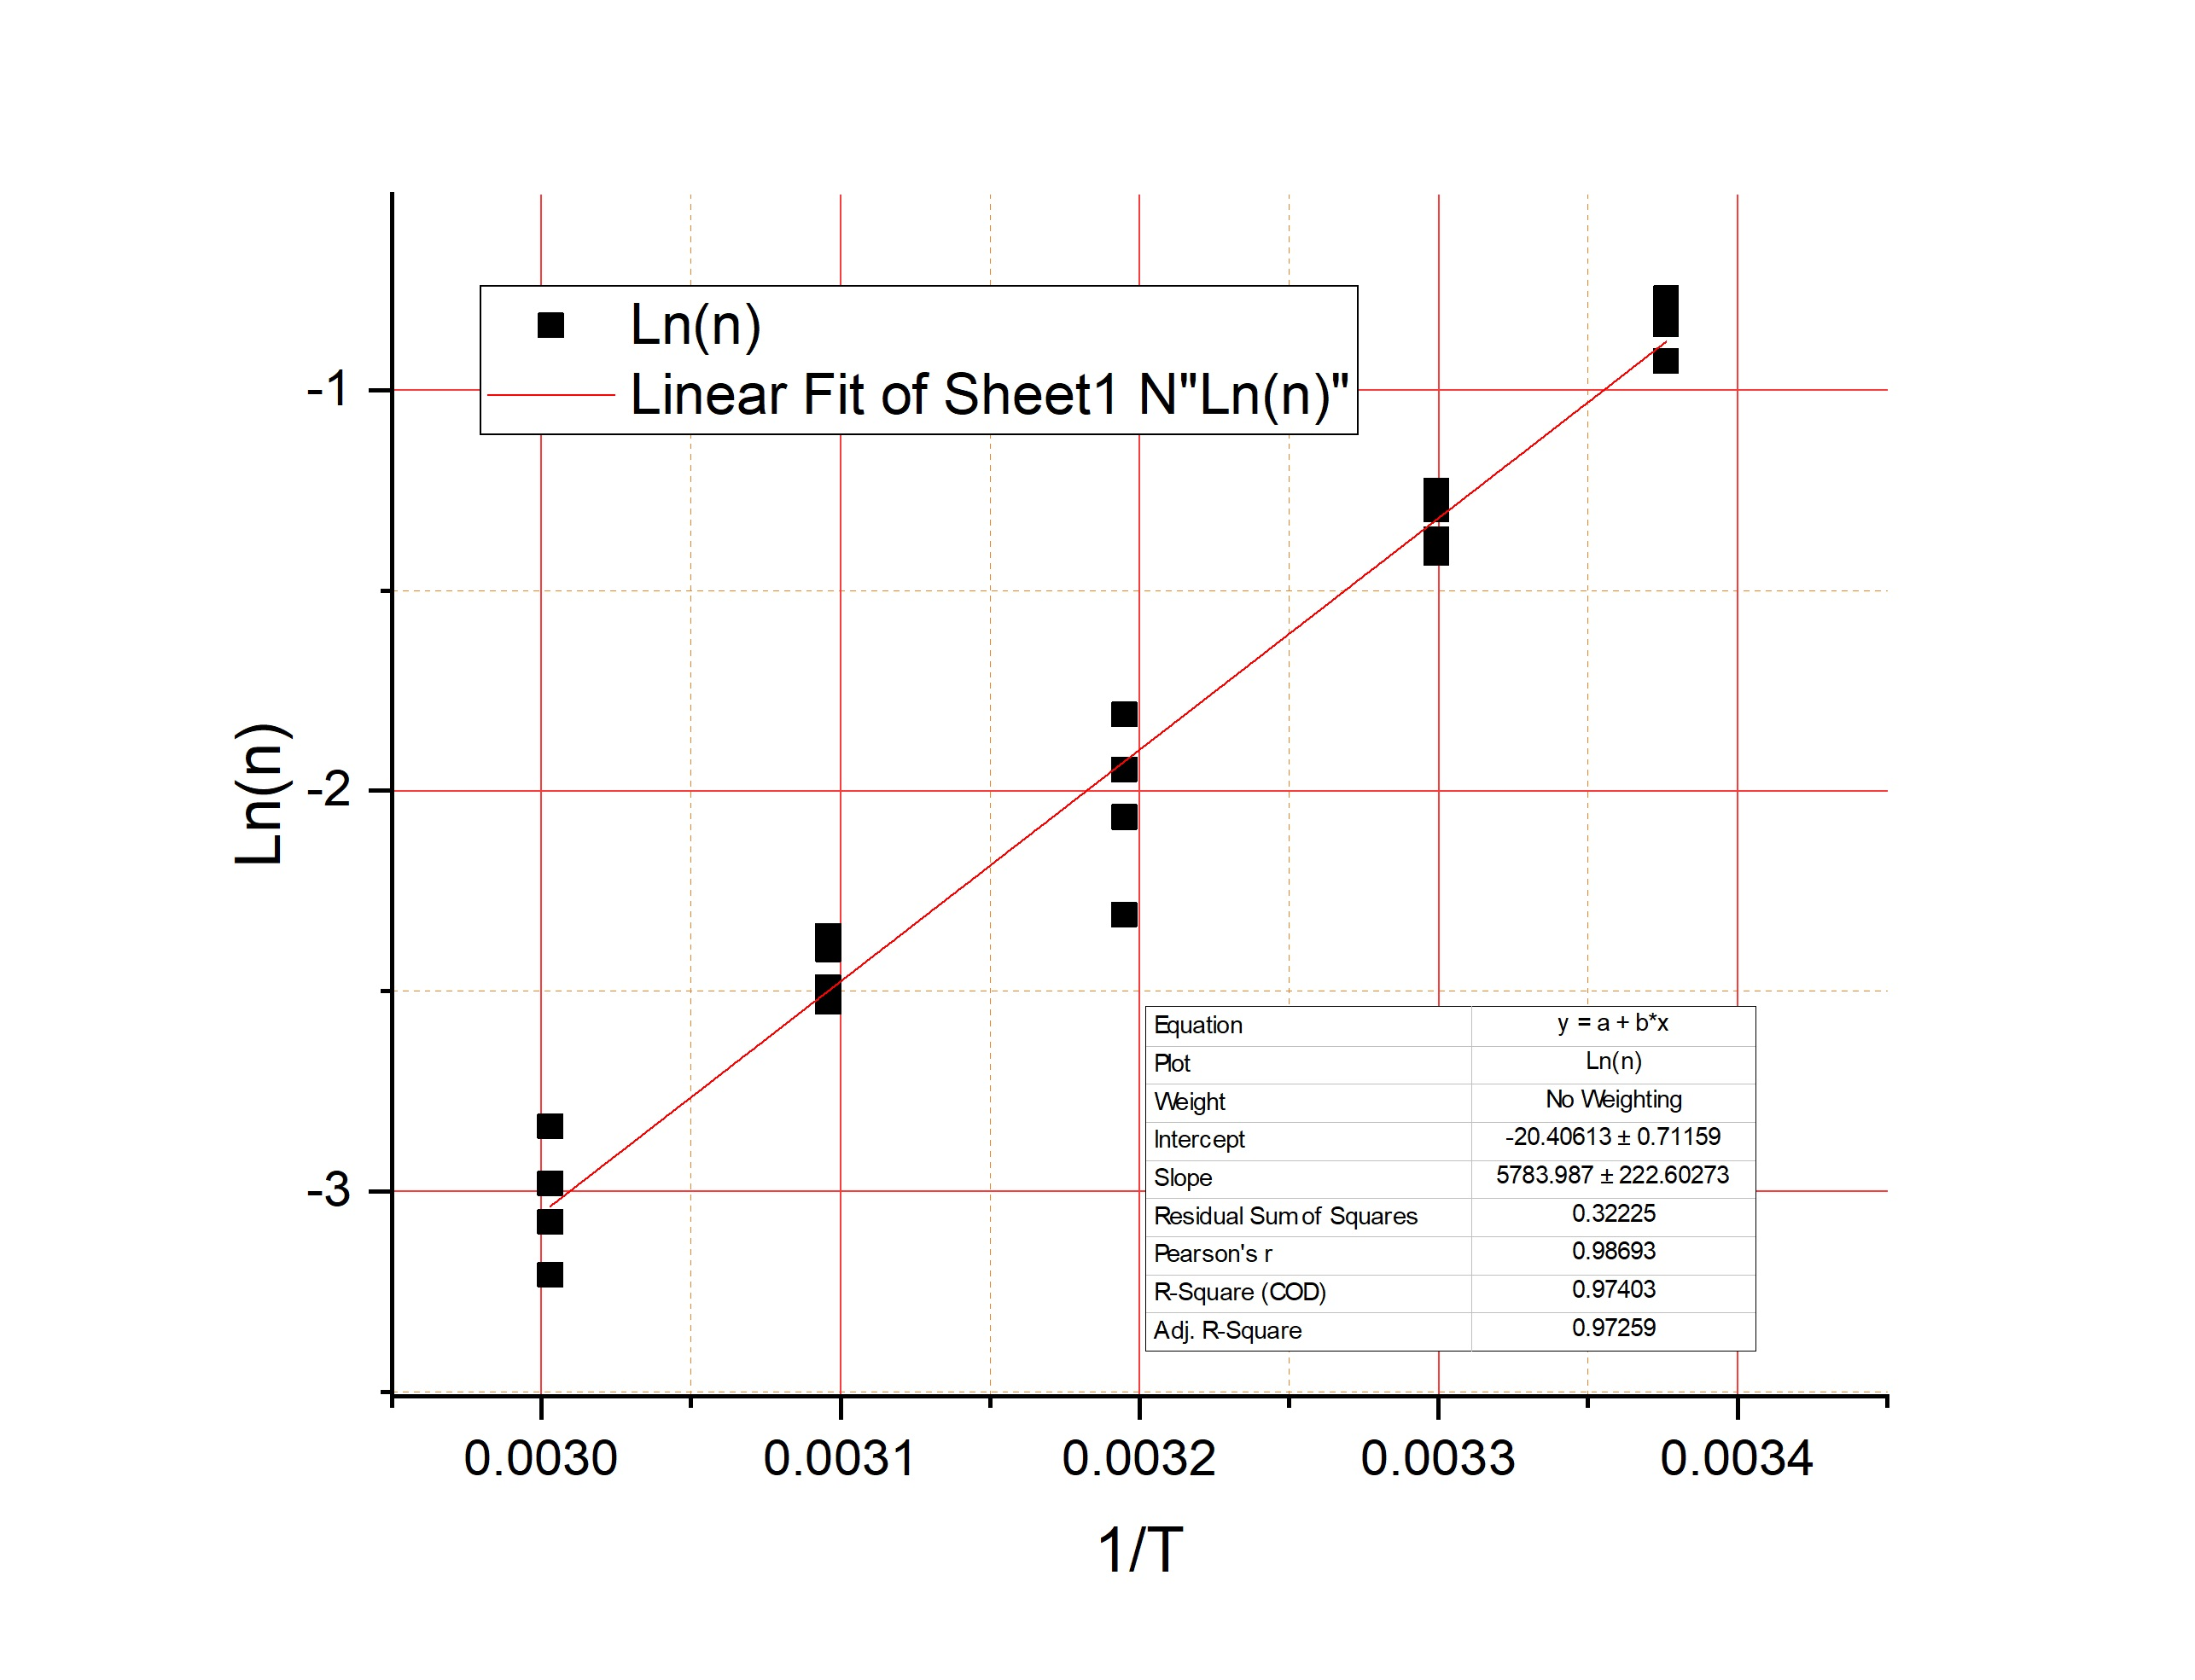
\includegraphics[scale=0.25]{1}
\caption{График зависимости $Ln(\eta)$ от $1/T$}
\label{gr}
\end{figure}
Как видно из информации на графике \ref{gr}, $k = 5784\pm 223$. 
Тогда определим энергию активации из формулы \ref{nrg}, а погрешность найдём по формуле 
\begin{equation}
\sigma_W = W \frac{\sigma_k}{k}
\end{equation}

Таким образом, $W=79*10^{-21}\pm 3*10^{-21}$
\section{Вывод}
В ходе этой работы по установившейся скорости падения шариков в жидкости установили её вязкость по формуле Стокса, в зависимости от температуры, проанализировав применимость формулы в каждом опыте; а также определили энергию активации молекул глицерина.

\end{document}
